\documentclass{article}




\usepackage{fullpage}
\usepackage{nopageno}
\usepackage{amsmath}
\usepackage{amsfonts}
\usepackage{graphicx}
\usepackage{framed}
\usepackage{xcolor}

\definecolor{dark_red}{rgb}{0.5,0.0,0.0}
\definecolor{dark_green}{rgb}{0.0,0.5,0.0}
\definecolor{dark_blue}{rgb}{0.0,0.0,0.5}
\definecolor{blue}{rgb}{0.0,0.0,1.0}

\newcommand{\dr}[1]{\textcolor{dark_red}{#1}}
\newcommand{\dg}[1]{\textcolor{dark_green}{#1}}
\newcommand{\db}[1]{\textcolor{dark_blue}{#1}}
\newcommand{\blue}[1]{\textcolor{blue}{#1}}



\begin{document}


\section*{Computing coefficients of linear combinations}

\textbf{Examples:}
\begin{itemize}
%%%%%%%%%%%%%%%%%%%%%%%%%%%%%
\item Let \(\mathbf{u} = \begin{bmatrix} 2 \\ -1 \\ 4 \end{bmatrix}\), \(\mathbf{v} = \begin{bmatrix} 3 \\ -1 \\ 5 \end{bmatrix}\), and \(\mathbf{w} = \begin{bmatrix} 0 \\ -1 \\ 2 \end{bmatrix}\). We will find scalars \(s\) and \(t\), provided they exist, that express \(\mathbf{w}\) as linear combination of \(\mathbf{u}\) and \(\mathbf{v}\):
\[\mathbf{w} = s\mathbf{u} + t\mathbf{v}\]
This equation is equivalent to:
\begin{align*}
& \begin{bmatrix} 0 \\ -1 \\ 2 \end{bmatrix} = s\begin{bmatrix} 2 \\ -1 \\ 4 \end{bmatrix} + t\begin{bmatrix} 3 \\ -1 \\ 5 \end{bmatrix} 
\iff \begin{bmatrix} 2s + 3t \\ -s - t \\ 4s + 5t \end{bmatrix} = \begin{bmatrix} 0 \\ -1 \\ 2 \end{bmatrix} 
\iff \left\{\begin{array}{c} 2s + 3t = 0 \\ -s - t = -1 \\ 4s + 5t = 2 \end{array}\right.
\end{align*}
Solving the first equation for \(t\) gives:
\[2s + 3t = 0 \iff 3t = -2s \iff t = -(2/3)s\]
Replacing \(t\) in the second and third equation gives:
\begin{align*}
& \left\{\begin{array}{c} -s - t = -1 \\ 4s + 5t = 2 \end{array}\right. 
\iff \left\{\begin{array}{c} -s - (-(2/3)s) = -1 \\ 4s + 5(-(2/3)s) = 2 \end{array}\right. 
\iff \left\{\begin{array}{c} -(1/3)s = -1 \\ (2/3)s = 2 \end{array}\right.  
\end{align*} 
Solving the second equation for \(s\) gives:
\[-(1/3)s = -1 \iff s = 3\]
Replacing \(s\) in the third equation gives:
\[(2/3)s = 2 \iff (2/3)(3) = 2 \iff 2 = 2\]
This equation is a tautology, brings no new information, and could henceforth be ignored. With the knowledge that \(t = -(2/3)s\) and \(s = 3\), replacing \(s\) in the expression for \(t\) gives:
\(t = -2\). Therefore:
\[s = 3 \quad\text{and}\quad t = -2\]  
satisfy
\[\mathbf{w} = s\mathbf{u} + t\mathbf{v}\]
%%%%%%%%%%%%%%%%%%%%%%%%%%%%%
\item Let \(\mathbf{u} = \begin{bmatrix} 0 \\ -1 \\ 3 \end{bmatrix}\), \(\mathbf{v} = \begin{bmatrix} 2 \\ 1 \\ -5 \end{bmatrix}\), and \(\mathbf{w} = \begin{bmatrix} 8 \\ -3 \\ 1 \end{bmatrix}\). We will find scalars \(s\) and \(t\), provided they exist, that express \(\mathbf{w}\) as linear combination of \(\mathbf{u}\) and \(\mathbf{v}\):
\[\mathbf{w} = s\mathbf{u} + t\mathbf{v}\]
This equation is equivalent to:
\begin{align*}
& \begin{bmatrix} 8 \\ -3 \\ 1 \end{bmatrix} = s\begin{bmatrix} 0 \\ -1 \\ 3 \end{bmatrix} + t\begin{bmatrix} 2 \\ 1 \\ -5 \end{bmatrix} 
\iff \begin{bmatrix} 2t \\ -s + t \\ 3s - 5t \end{bmatrix} = \begin{bmatrix} 8 \\ -3 \\ 1 \end{bmatrix}  
\iff \left\{\begin{array}{c} 2t = 8 \\ -s + t = -3 \\ 3s - 5t = 1 \end{array}\right.
\end{align*}
Solving the first equation for \(t\) gives:
\[2t = 8 \iff t = 4\]
Replacing \(t\) in the second and third equation gives:
\begin{align*}
& \left\{\begin{array}{c} -s + t = -3 \\ 3s - 5t = 1 \end{array} \right.
\iff \left\{\begin{array}{c} -s + 4 = -3 \\ 3s - 5(4) = 1 \end{array} \right. 
\iff \left\{\begin{array}{c} -s + 4 = -3 \\ 3s - 20 = 1 \end{array} \right. 
\end{align*}
Solving the second equation for \(s\) gives:
\[-s + 4 = -3 \iff -s = -7 \iff s = 7\]
Replacing \(s\) in the third equation gives:
\[3s - 20 = 1 \iff 3(7) - 20 = 1 \iff 1 = 1\]
This equation is a tautology, brings no new information, and could henceforth be ignored. In summary, 
\[s = 7 \quad\text{and}\quad t = 4\]
which satisfy
\[\mathbf{w} = s\mathbf{u} + t\mathbf{v}\]
%%%%%%%%%%%%%%%%%%%%%%%%%%%%%
\item Let \(\mathbf{u} = \begin{bmatrix} -1 \\ 7 \\ 5 \end{bmatrix}\), \(\mathbf{v} = \begin{bmatrix} 4 \\ 0 \\ -9 \end{bmatrix}\), and \(\mathbf{w} = \begin{bmatrix} 10 \\ 14 \\ -16 \end{bmatrix}\). We will find scalars \(s\) and \(t\), provided they exist, that express \(\mathbf{w}\) as linear combination of \(\mathbf{u}\) and \(\mathbf{v}\):
\[\mathbf{w} = s\mathbf{u} + t\mathbf{v}\]
This equation is equivalent to: 
\begin{align*}
& \begin{bmatrix} 10 \\ 14 \\ -16 \end{bmatrix} = s\begin{bmatrix} -1 \\ 7 \\ 5 \end{bmatrix} + t\begin{bmatrix} 4 \\ 0 \\ -9 \end{bmatrix}  
\iff \begin{bmatrix} -s + 4t \\ 7s \\ 5s - 9t \end{bmatrix} = \begin{bmatrix} 10 \\ 14 \\ -16 \end{bmatrix}  
\iff \left\{\begin{array}{c} -s + 4t = 10 \\ 7s = 14 \\ 5s - 9t = -16 \end{array}\right.
\end{align*}
Solving the second equation for \(s\) gives:
\[7s = 14 \iff s = 2\]
Replacing \(s\) in the first and third equation gives:
\begin{align*}
& \left\{\begin{array}{c} -s + 4t = 10 \\ 5s - 9t = -16 \end{array}\right. 
\iff \left\{\begin{array}{c} -2 + 4t = 10 \\ 5(2) - 9t = -16 \end{array}\right.   
\iff \left\{\begin{array}{c} -2 + 4t = 10 \\ 10 - 9t = -16 \end{array}\right.   
\end{align*}
Solving the first equation for \(t\) gives:
\[-2 + 4t = 10 \iff 4t = 12 \iff t = 3\]
Replacing \(t\) in the third equation gives:
\[10 - 9t = -16 \iff 10 - 9(3) = -16 \iff -17 = -16\]
This equation is a contradiction, and due to this contradiction, the system of equations has no solution. The coefficients \(s\) and \(t\) cannot exist, and \(\mathbf{w}\) cannot be expressed as a linear combination of \(\mathbf{u}\) and \(\mathbf{v}\):
\[\mathbf{w} \neq s\mathbf{u} + t\mathbf{v}\]
\end{itemize}




\section*{Vector and parametric equations}

Before now, curves and surfaces are quantified by listing one or multiple equations that all points on the curve or surface must satisfy. Now, additional variables, referred to as {\bf parameters}, will be used to quantify curves and surfaces. With a parametric curve or surface, each coordinate is an explicit function of the parameter variables. Each assignment to the parameter values, from the domain of valid parameter values, will generate a point that lies on the curve or surface. 

When a set of equations is listed, a point can be arbitrarily chosen, and then determined as to whether the point lies on the curve/surface or not. 

When parametric equations are used, points can be generated directly by setting the parameter values as opposed to choosing a point and then ``testing" whether the point is on the curve or not.

Two ``forms" of parametric equations will be addressed:
\begin{itemize}
\item A vector equation is a parametric equation, where the position vector of the generated point is expressed as an expression involving vectors and the parameters.
\item A basic set of parametric equations for a set of points in space has an independent expression for each coordinate. The parameters are shared between the expressions however.
\end{itemize}



\section*{The equations of lines}

\begin{tabular}{cc}
\parbox{0.5\textwidth}{
Consider an arbitrary point \(P_0\) with position vector \(\mathbf{q}_0 = \begin{bmatrix} x_0 \\ y_0 \\ z_0 \end{bmatrix}\) and a nonzero direction vector \(\mathbf{v} = \begin{bmatrix} v_x \\ v_y \\ v_z \end{bmatrix}\). With regards to a line that passes through point \(P_0\) and is parallel to vector \(\mathbf{v}\), one possible vector equation of the line is:
\[\mathbf{q}(t) = \mathbf{q}_0 + \mathbf{v}t\]
In this case, \(t = 0\) generates the point \(P_0\). 
} & \parbox{0.5\textwidth}{
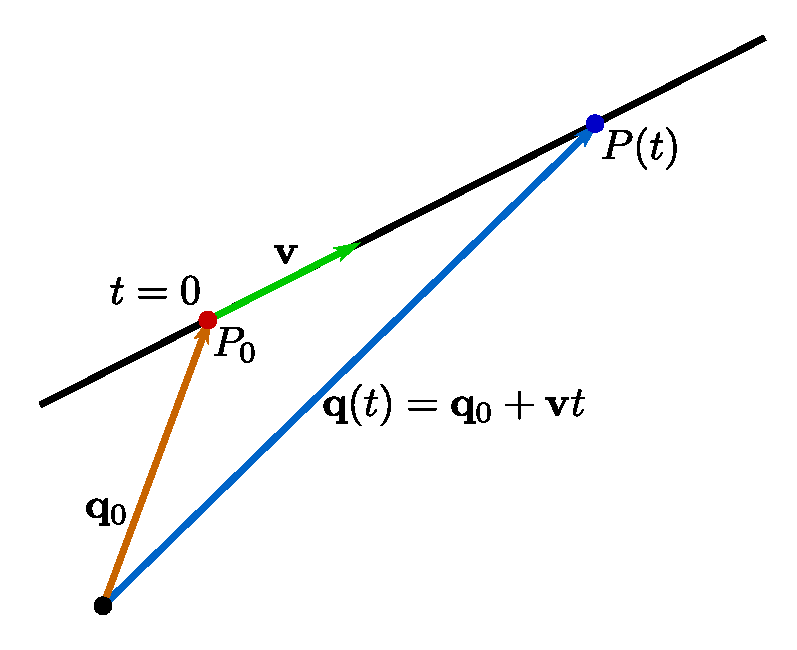
\includegraphics[width = 0.5\textwidth]{vector_equation_line}
}
\end{tabular}
The parametric equations themselves are:
\begin{align*}
& \begin{bmatrix} x(t) \\ y(t) \\ z(t) \end{bmatrix} = \begin{bmatrix} x_0 \\ y_0 \\ z_0 \end{bmatrix} + \begin{bmatrix} v_x \\ v_y \\ v_z \end{bmatrix}t = \begin{bmatrix} x_0 + v_x t \\ y_0 + v_y t \\ z_0 + v_z t \end{bmatrix} 
\iff \left\{\begin{array}{c} x(t) = x_0 + v_x t \\ y(t) = y_0 + v_y t \\ z(t) = z_0 + v_z t \end{array}\right.
\end{align*}

It should be noted that parametric equations are not unique. The same curve/surface may have different parametric equations where the same value of \(t\) will generate different points. As an example, consider the line \(L\) that passes through a point with position vector \(\mathbf{q}_0\) and is parallel to vector \(\mathbf{v}\). This, as discussed above, yields the vector equation \(\mathbf{q}(t) = \mathbf{q}_0 + \mathbf{v}t\). Line \(L\) also passes through the point with position vector \(\mathbf{q}_0 - 3\mathbf{v}\), and is parallel to the vector \(-5\mathbf{v}\). This yields the vector equation \(\mathbf{q}(t) = (\mathbf{q}_0 - 3\mathbf{v}) - 5\mathbf{v}t\) which yields a different set of parametric equations.

\begin{tabular}{cc}
\parbox{0.5\textwidth}{
The line {\bf segment} from point \(P_0\) with position vector \(\mathbf{q}_0 = \begin{bmatrix} x_0 \\ y_ 0 \\ z_0 \end{bmatrix}\) to point \(P_1\) with position vector \(\mathbf{q}_1 = \begin{bmatrix} x_1 \\ y_1 \\ z_1 \end{bmatrix}\) has the vector equation:   
\[\mathbf{q}(t) = \mathbf{q}_0 + (\mathbf{q}_1 - \mathbf{q}_0)t  = (1 - t)\mathbf{q}_0 + t \mathbf{q}_1\]
The parameter \(t\) is confined to the interval \([0, 1]\). When \(t = 0\), \(\mathbf{q}(0) = \mathbf{q}_0\). When \(t = 1\), \(\mathbf{q}(1) = \mathbf{q}_1\). 
} & \parbox{0.5\textwidth}{
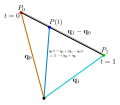
\includegraphics[width = 0.5\textwidth]{vector_equation_line_segment}
}
\end{tabular}
The parametric equations themselves are:
\[\left\{\begin{array}{c} x(t) = x_0 + (x_1 - x_0)t = (1 - t)x_0 + t x_1 \\ y(t) = y_0 + (y_1 - y_0)t = (1 - t)y_0 + t y_1 \\ z(t) = z_0 + (z_1 - z_0)t = (1 - t)z_0 + t z_1\end{array}\right. \quad (0 \leq t \leq 1)\]
The parameter \(t\) is confined to the interval \([0, 1]\).

\textbf{Examples:}
\begin{itemize}
%%%%%%%%%%%%%%%%%%%%%%%%%%%
\item Given the points \(X(7, 1, -5)\) and \(Y(2, -3, -6)\), the line that passes through \(X\) and \(Y\) must be parallel to \(\overrightarrow{XY} = \begin{bmatrix} 2 - 7 \\ (-3) - 1 \\ (-6) - (-5) \end{bmatrix} = \begin{bmatrix} -5 \\ -4 \\ -1 \end{bmatrix}\). One possible vector equation is:
\[\mathbf{q}(t) = \begin{bmatrix} 7 \\ 1 \\ -5 \end{bmatrix} + \begin{bmatrix} -5 \\ -4 \\ -1 \end{bmatrix}t\] 
The corresponding set of parametric equations is: 
\[\left\{\begin{array}{c} x(t) = 7 - 5t \\ y(t) = 1 - 4t \\ z(t) = -5 - t \end{array}\right.\]
Another set of parametric equations can be derived by observing that the line passes through the point where \(t = 2\): \(\mathbf{q}(2) = \begin{bmatrix} -3 \\ -7 \\ -7 \end{bmatrix}\), and is parallel to the vector \(-3\overrightarrow{XY} = \begin{bmatrix} 15 \\ 12 \\ 3 \end{bmatrix}\) Another vector equation {\bf of the same line} is: 
\[\mathbf{q}(t) = \begin{bmatrix} -3 \\ -7 \\ -7 \end{bmatrix} + \begin{bmatrix} 15 \\ 12 \\ 3 \end{bmatrix}t\] 
The corresponding set of parametric equations is: 
\[\left\{\begin{array}{c} x(t) = -3 + 15t \\ y(t) = -7 + 12t \\ z(t) = -7 + 3t \end{array}\right.\]
%%%%%%%%%%%%%%%%%%%%%%%%%%%
\item Given the points \(B(8, 1, -2)\) and \(A(1, -7, 3)\), the line that passes through \(B\) and \(A\) must be parallel to \(\overrightarrow{BA} = \begin{bmatrix} 1 - 8 \\ (-7) - 1 \\ 3 - (-2) \end{bmatrix} = \begin{bmatrix} -7 \\ -8 \\ 5 \end{bmatrix}\). One possible vector equation is:
\[\mathbf{q}(t) = \begin{bmatrix} 8 \\ 1 \\ -2 \end{bmatrix} + \begin{bmatrix} -7 \\ -8 \\ 5 \end{bmatrix}t\]
The corresponding set of parametric equations is: 
\[\left\{\begin{array}{c} x(t) = 8 - 7t \\ y(t) = 1 - 8t \\ z(t) = -2 + 5t \end{array}\right.\]
%%%%%%%%%%%%%%%%%%%%%%%%%%%
\item Given the points \(M(0, -7, 2)\) and \(C(4, 5, 0)\), the line that passes through \(M\) and \(C\) must be parallel to \(\overrightarrow{MC} = \begin{bmatrix} 4 - 0 \\ 5 - (-7) \\ 0 - 2 \end{bmatrix} = \begin{bmatrix} 4 \\ 12 \\ -2 \end{bmatrix}\). One possible vector equation is:
\[\mathbf{q}(t) = \begin{bmatrix} 0 \\ -7 \\ 2 \end{bmatrix} + \begin{bmatrix} 4 \\ 12 \\ -2 \end{bmatrix}t\]
The corresponding set of parametric equations is:
\[\left\{\begin{array}{c} x(t) = 4t \\ y(t) = -7 + 12t \\ z(t) = 2 - 2t \end{array}\right.\]
\end{itemize}



\section*{The equations of planes}

\begin{tabular}{cc}
\parbox{0.5\textwidth}{
Consider an arbitrary point \(P_0\) with position vector \(\mathbf{q}_0\) and two nonzero vectors \(\mathbf{v}_1\) and \(\mathbf{v}_2\) that are {\bf not parallel}.
one possible vector equation of the plane is:
\begin{align*}
& \mathbf{q}(t_1, t_2) = \mathbf{q}_0 + \mathbf{v}_1 t_1 + \mathbf{v}_2 t_2 = 
\end{align*}
} & \parbox{0.5\textwidth}{
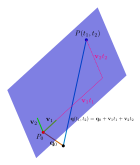
\includegraphics[width = 0.5\textwidth]{vector_equation_plane}
}
\end{tabular}
The parametric equations themselves are:
\[\begin{bmatrix} x(t) \\ y(t) \\ z(t) \end{bmatrix} = \begin{bmatrix} x_0 \\ y_0 \\ z_0 \end{bmatrix} + \begin{bmatrix} v_{1x} \\ v_{1y} \\ v_{1z} \end{bmatrix}t_1 + \begin{bmatrix} v_{2x} \\ v_{2y} \\ v_{2z} \end{bmatrix}t_2 = \begin{bmatrix} x_0 + v_{1x} t_1 + v_{2x} t_2 \\ y_0 + v_{1y} t_1 + v_{2y} t_2 \\ z_0 + v_{1z} t_1 + v_{2z} t_2 \end{bmatrix}  
\iff \left\{\begin{array}{c} x(t) = x_0 + v_{1x} t_1 + v_{2x} t_2 \\ y(t) = y_0 + v_{1y} t_1 + v_{2y} t_2 \\ z(t) = z_0 + v_{1z} t_1 + v_{2z} t_2 \end{array}\right.\]

\textbf{Examples:}
\begin{itemize}
%%%%%%%%%%%%%%%%%%%%%%%%%%%
\item Given the points \(T(6, -1, 0)\), \(D(10, -4, -7)\), and \(Q(-1, 0, 2)\) the plane that passes through the points \(T\), \(D\), and \(Q\) must be parallel to \(\overrightarrow{TD} = \begin{bmatrix} 10 - 6 \\ (-4) - (-1) \\ (-7) - 0 \end{bmatrix} = \begin{bmatrix} 4 \\ -3 \\ -7 \end{bmatrix}\) and \(\overrightarrow{TQ} = \begin{bmatrix} (-1) - 6 \\ 0 - (-1) \\ 2 - 0 \end{bmatrix} = \begin{bmatrix} -7 \\ 1 \\ 2 \end{bmatrix}\). One possible vector equation is:
\[\mathbf{q}(t_1, t_2) = \begin{bmatrix} 6 \\ -1 \\ 0 \end{bmatrix} + \begin{bmatrix} 4 \\ -3 \\ -7 \end{bmatrix}t_1 + \begin{bmatrix} -7 \\ 1 \\ 2 \end{bmatrix}t_2\] 
The corresponding set of parametric equations is: 
\[\left\{\begin{array}{c} x(t_1, t_2) = 6 + 4t_1 - 7t_2 \\ y(t_1, t_2) = -1 - 3t_1 + t_2 \\ z(t_1, t_2) = -7t_1 + 2t_2 \end{array}\right.\]
Another set of parametric equations can be derived by observing that the plane passes through the point where \(t_1 = -1\) and \(t_2 = 3\): \(\mathbf{q}(-1, 3) = \begin{bmatrix} -19 \\ 5 \\ 13 \end{bmatrix}\), and is parallel to the vectors \(2\overrightarrow{TD} = \begin{bmatrix} 8 \\ -6 \\ -14 \end{bmatrix}\) and \(\overrightarrow{TD} - 3\overrightarrow{TQ} = \begin{bmatrix}  25 \\ -6 \\ -13 \end{bmatrix}\) Another vector equation {\bf of the same plane} is: 
\[\mathbf{q}(t) = \begin{bmatrix} -19 \\ 5 \\ 13 \end{bmatrix} + \begin{bmatrix} 8 \\ -6 \\ -14 \end{bmatrix}t_1 + \begin{bmatrix} 25 \\ -6 \\ -13 \end{bmatrix}t_2\] 
The corresponding set of parametric equations is: 
\[\left\{\begin{array}{c} x(t_1, t_2) = -19 + 8t_1 + 25t_2 \\ y(t_1, t_2) = 5 - 6t_1 - 6t_2 \\ z(t_1, t_2) = 13 - 14t_1 - 13t_2 \end{array}\right.\]
%%%%%%%%%%%%%%%%%%%%%%%%%%%
\item Given the points \(R(-1, -3, -4)\), \(A(-1, 2, 3)\), and \(N(6, 2, 7)\) the plane that passes through the points \(R\), \(A\), and \(N\) must be parallel to \(\overrightarrow{RA} = \begin{bmatrix} (-1) - (-1) \\ 2 - (-3) \\ 3 - (-4) \end{bmatrix} = \begin{bmatrix} 0 \\ 5 \\ 7 \end{bmatrix}\) and \(\overrightarrow{RN} = \begin{bmatrix} 6 - (-1) \\ 2 - (-3) \\ 7 - (-4) \end{bmatrix} = \begin{bmatrix} 7 \\ 5 \\ 11 \end{bmatrix}\). One possible vector equation is:
\[\mathbf{q}(t_1, t_2) = \begin{bmatrix} -1 \\ -3 \\ -4 \end{bmatrix} + \begin{bmatrix} 0 \\ 5 \\ 7 \end{bmatrix}t_1 + \begin{bmatrix} 7 \\ 5 \\ 11 \end{bmatrix}t_2\] 
The corresponding set of parametric equations is: 
\[\left\{\begin{array}{c} x(t_1, t_2) = -1 + 7t_2 \\ y(t_1, t_2) = -3 + 5t_1 + 5t_2 \\ z(t_1, t_2) = -4 + 7t_1 + 11t_2 \end{array}\right.\]
%%%%%%%%%%%%%%%%%%%%%%%%%%%
\item Given the points \(Y(11, 8, -2)\), \(P(7, 11, -5)\), and \(S(13, 7, -5)\) the plane that passes through the points \(Y\), \(P\), and \(S\) must be parallel to \(\overrightarrow{YP} = \begin{bmatrix} 7 - 11 \\ 11 - 8 \\ (-5) - (-2) \end{bmatrix} = \begin{bmatrix} -4 \\ 3 \\ -3 \end{bmatrix}\) and \(\overrightarrow{YS} = \begin{bmatrix} 13 - 11 \\ 7 - 8 \\ (-5) - (-2) \end{bmatrix} = \begin{bmatrix} 2 \\ -1 \\ -3 \end{bmatrix}\). One possible vector equation is:
\[\mathbf{q}(t_1, t_2) = \begin{bmatrix} 11 \\ 8 \\ -2 \end{bmatrix} + \begin{bmatrix} -4 \\ 3 \\ -3 \end{bmatrix}t_1 + \begin{bmatrix} 2 \\ -1 \\ -3 \end{bmatrix}t_2\] 
The corresponding set of parametric equations is: 
\[\left\{\begin{array}{c} x(t_1, t_2) = 11 - 4t_1 + 2t_2 \\ y(t_1, t_2) = 8 + 3t_1 - t_2 \\ z(t_1, t_2) = -2 - 3t_1 - 3t_2 \end{array}\right.\]
\end{itemize}



\section*{Distance from a point to a line}

\begin{tabular}{cc}
\parbox{0.5\textwidth}{
Consider a line \(L\) and a point \(P\). If \(Q\) is the point on line \(L\) that is closest to point \(P\), then the line segment \(QP\) is perpendicular to line \(L\) as depicted on the right. The closest distance \(d\) between line \(L\) and point \(P\) is the distance between \(Q\) and \(P\). Let \(\mathbf{u}\) be an arbitrary vector that is parallel to line \(L\), and let \(R\) be an arbitrary point on line \(L\), not necessarily the closest point \(Q\). Let \(\mathbf{v}\) be the displacement \(\overrightarrow{RP}\). Since \(R\) is not necessarily point \(Q\), \(\mathbf{v} = \overrightarrow{RP}\) is not necessarily perpendicular to \(\mathbf{u}\). The displacement from \(Q\) to \(P\) is the component of \(\mathbf{v}\) that is perpendicular to \(\mathbf{u}\): \(\overrightarrow{QP} = \text{perp}(\mathbf{v}|\mathbf{u})\). The distance \(d\) is the length of this displacement:
\[d = \|\text{perp}(\mathbf{v}|\mathbf{u})\| = \frac{\sqrt{\|\mathbf{u}\|^2 \|\mathbf{v}\|^2 - (\mathbf{u} \bullet \mathbf{v})^2}}{\|\mathbf{u}\|}\] 
} & \parbox{0.5\textwidth}{
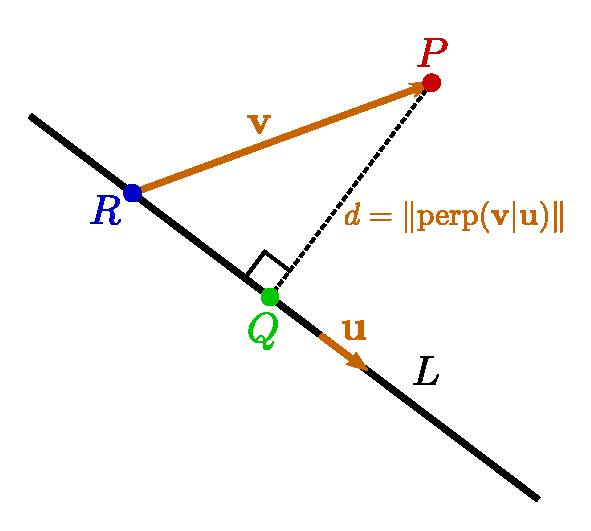
\includegraphics[width = 0.5\textwidth]{point_line_closest_distance}
}
\end{tabular}

\textbf{Example:}
\begin{itemize}
\item Consider the 3 points: \(A(6, -2, 3)\), \(B(4, -1, 2)\), and \(C(5, -4, 6)\). Let line \(L\) pass through points \(A\) and \(B\). The perpendicular distance \(d\) of point \(C\) from line \(L\) is what is sought. The vector \(\mathbf{u} = \overrightarrow{AB} = \begin{bmatrix} 4 - 6 \\ (-1) - (-2) \\ 2 - 3 \end{bmatrix} = \begin{bmatrix} -2 \\ 1 \\ -1 \end{bmatrix}\) is parallel to line \(L\). The vector \(\mathbf{v} = \overrightarrow{AC} = \begin{bmatrix} 5 - 6 \\ (-4) - (-2) \\ 6 - 3 \end{bmatrix} = \begin{bmatrix} -1 \\ -2 \\ 3 \end{bmatrix}\) connects a point on line \(L\) to point \(C\). The length of the component of \(\mathbf{v}\) that is perpendicular to line \(L\) is the perpendicular distance \(d\). We first compute:
\begin{itemize}
\item[*] \(\|\mathbf{u}\|^2 = \mathbf{u} \bullet \mathbf{u} = (-2)^2 + 1^2 + (-1)^2 = 4 + 1 + 1 = 6\)
\item[*] \(\|\mathbf{v}\|^2 = \mathbf{v} \bullet \mathbf{v} = (-1)^2 + (-2)^2 + 3^2 = 1 + 4 + 9 = 14\)
\item[*] \(\mathbf{u} \bullet \mathbf{v} = (-2)(-1) + (1)(-2) + (-1)(3) = 2 - 2 - 3 = -3\)
\end{itemize} 
We finally compute:
\[d = \frac{\sqrt{\|\mathbf{u}\|^2 \|\mathbf{v}\|^2 - (\mathbf{u} \bullet \mathbf{v})^2}}{\|\mathbf{u}\|}
= \frac{\sqrt{(6)(14) - (-3)^2}}{\sqrt{6}}
= \frac{\sqrt{84 - 9}}{\sqrt{6}} 
= \sqrt{\frac{75}{6}}
= \sqrt{\frac{25}{2}}
= \frac{5}{\sqrt{2}}\] 
\end{itemize}


\end{document}   















